\PassOptionsToPackage{unicode=true}{hyperref} % options for packages loaded elsewhere
\PassOptionsToPackage{hyphens}{url}
%
\documentclass[]{article}
\usepackage{lmodern}
\usepackage{amssymb,amsmath}
\usepackage{ifxetex,ifluatex}
\usepackage{fixltx2e} % provides \textsubscript
\ifnum 0\ifxetex 1\fi\ifluatex 1\fi=0 % if pdftex
  \usepackage[T1]{fontenc}
  \usepackage[utf8]{inputenc}
  \usepackage{textcomp} % provides euro and other symbols
\else % if luatex or xelatex
  \usepackage{unicode-math}
  \defaultfontfeatures{Ligatures=TeX,Scale=MatchLowercase}
\fi
% use upquote if available, for straight quotes in verbatim environments
\IfFileExists{upquote.sty}{\usepackage{upquote}}{}
% use microtype if available
\IfFileExists{microtype.sty}{%
\usepackage[]{microtype}
\UseMicrotypeSet[protrusion]{basicmath} % disable protrusion for tt fonts
}{}
\IfFileExists{parskip.sty}{%
\usepackage{parskip}
}{% else
\setlength{\parindent}{0pt}
\setlength{\parskip}{6pt plus 2pt minus 1pt}
}
\usepackage{hyperref}
\hypersetup{
            pdfborder={0 0 0},
            breaklinks=true}
\urlstyle{same}  % don't use monospace font for urls
\usepackage{color}
\usepackage{fancyvrb}
\newcommand{\VerbBar}{|}
\newcommand{\VERB}{\Verb[commandchars=\\\{\}]}
\DefineVerbatimEnvironment{Highlighting}{Verbatim}{commandchars=\\\{\}}
% Add ',fontsize=\small' for more characters per line
\newenvironment{Shaded}{}{}
\newcommand{\AlertTok}[1]{\textcolor[rgb]{1.00,0.00,0.00}{\textbf{#1}}}
\newcommand{\AnnotationTok}[1]{\textcolor[rgb]{0.38,0.63,0.69}{\textbf{\textit{#1}}}}
\newcommand{\AttributeTok}[1]{\textcolor[rgb]{0.49,0.56,0.16}{#1}}
\newcommand{\BaseNTok}[1]{\textcolor[rgb]{0.25,0.63,0.44}{#1}}
\newcommand{\BuiltInTok}[1]{#1}
\newcommand{\CharTok}[1]{\textcolor[rgb]{0.25,0.44,0.63}{#1}}
\newcommand{\CommentTok}[1]{\textcolor[rgb]{0.38,0.63,0.69}{\textit{#1}}}
\newcommand{\CommentVarTok}[1]{\textcolor[rgb]{0.38,0.63,0.69}{\textbf{\textit{#1}}}}
\newcommand{\ConstantTok}[1]{\textcolor[rgb]{0.53,0.00,0.00}{#1}}
\newcommand{\ControlFlowTok}[1]{\textcolor[rgb]{0.00,0.44,0.13}{\textbf{#1}}}
\newcommand{\DataTypeTok}[1]{\textcolor[rgb]{0.56,0.13,0.00}{#1}}
\newcommand{\DecValTok}[1]{\textcolor[rgb]{0.25,0.63,0.44}{#1}}
\newcommand{\DocumentationTok}[1]{\textcolor[rgb]{0.73,0.13,0.13}{\textit{#1}}}
\newcommand{\ErrorTok}[1]{\textcolor[rgb]{1.00,0.00,0.00}{\textbf{#1}}}
\newcommand{\ExtensionTok}[1]{#1}
\newcommand{\FloatTok}[1]{\textcolor[rgb]{0.25,0.63,0.44}{#1}}
\newcommand{\FunctionTok}[1]{\textcolor[rgb]{0.02,0.16,0.49}{#1}}
\newcommand{\ImportTok}[1]{#1}
\newcommand{\InformationTok}[1]{\textcolor[rgb]{0.38,0.63,0.69}{\textbf{\textit{#1}}}}
\newcommand{\KeywordTok}[1]{\textcolor[rgb]{0.00,0.44,0.13}{\textbf{#1}}}
\newcommand{\NormalTok}[1]{#1}
\newcommand{\OperatorTok}[1]{\textcolor[rgb]{0.40,0.40,0.40}{#1}}
\newcommand{\OtherTok}[1]{\textcolor[rgb]{0.00,0.44,0.13}{#1}}
\newcommand{\PreprocessorTok}[1]{\textcolor[rgb]{0.74,0.48,0.00}{#1}}
\newcommand{\RegionMarkerTok}[1]{#1}
\newcommand{\SpecialCharTok}[1]{\textcolor[rgb]{0.25,0.44,0.63}{#1}}
\newcommand{\SpecialStringTok}[1]{\textcolor[rgb]{0.73,0.40,0.53}{#1}}
\newcommand{\StringTok}[1]{\textcolor[rgb]{0.25,0.44,0.63}{#1}}
\newcommand{\VariableTok}[1]{\textcolor[rgb]{0.10,0.09,0.49}{#1}}
\newcommand{\VerbatimStringTok}[1]{\textcolor[rgb]{0.25,0.44,0.63}{#1}}
\newcommand{\WarningTok}[1]{\textcolor[rgb]{0.38,0.63,0.69}{\textbf{\textit{#1}}}}
\usepackage{graphicx,grffile}
\makeatletter
\def\maxwidth{\ifdim\Gin@nat@width>\linewidth\linewidth\else\Gin@nat@width\fi}
\def\maxheight{\ifdim\Gin@nat@height>\textheight\textheight\else\Gin@nat@height\fi}
\makeatother
% Scale images if necessary, so that they will not overflow the page
% margins by default, and it is still possible to overwrite the defaults
% using explicit options in \includegraphics[width, height, ...]{}
\setkeys{Gin}{width=\maxwidth,height=\maxheight,keepaspectratio}
\setlength{\emergencystretch}{3em}  % prevent overfull lines
\providecommand{\tightlist}{%
  \setlength{\itemsep}{0pt}\setlength{\parskip}{0pt}}
\setcounter{secnumdepth}{0}
% Redefines (sub)paragraphs to behave more like sections
\ifx\paragraph\undefined\else
\let\oldparagraph\paragraph
\renewcommand{\paragraph}[1]{\oldparagraph{#1}\mbox{}}
\fi
\ifx\subparagraph\undefined\else
\let\oldsubparagraph\subparagraph
\renewcommand{\subparagraph}[1]{\oldsubparagraph{#1}\mbox{}}
\fi

% set default figure placement to htbp
\makeatletter
\def\fps@figure{htbp}
\makeatother


\date{}

\begin{document}

\textbf{IB031 Project}

\begin{itemize}
\item
  \href{https://www.kaggle.com/altruistdelhite04/loan-prediction-problem-dataset}{Source}
\item
  \href{https://www.kaggle.com/altruistdelhite04/loan-prediction-problem-dataset/download/evL45lGV3RssadtbrRzN\%2Fversions\%2FvfUNmIbaXE87YsRW0vw8\%2Ffiles\%2Ftest_Y3wMUE5_7gLdaTN.csv?datasetVersionNumber=1}{Testing
  csv}
\item
  \href{https://www.kaggle.com/altruistdelhite04/loan-prediction-problem-dataset/download/evL45lGV3RssadtbrRzN\%2Fversions\%2FvfUNmIbaXE87YsRW0vw8\%2Ffiles\%2Ftrain_u6lujuX_CVtuZ9i.csv?datasetVersionNumber=1}{Training
  csv}
\end{itemize}

In this project we will implement several models to predict credibility
of a loan applicant. We will use the Loan Prediction Problem Dataset
from Kaggle. The structure of the project is as follows:

\begin{enumerate}
\def\labelenumi{\arabic{enumi}.}
\tightlist
\item
  \protect\hyperlink{1-exploratory-analysis}{Exploratory Analysis}
\item
  \protect\hyperlink{2-data-preprocessing}{Preprocessing of the dataset}
\item
  \protect\hyperlink{3-naive-baseline-model}{Naive classifier}
\item
  \protect\hyperlink{4-decision-tree-classifier}{Decision tree
  classifier}
\item
  \protect\hyperlink{5-knn-classifier}{KNN classifier}
\item
  \protect\hyperlink{6-support-vector-machine}{Support Vector Machine}
\item
  \protect\hyperlink{7-deep-neural-network}{Deep Neural Network}
\item
  \protect\hyperlink{8-evaluation}{Evaluation}
\item
  \protect\hyperlink{9-conclusion}{Conclusion}
\end{enumerate}

\hypertarget{exploratory-analysis}{%
\subsection{1. Exploratory Analysis}\label{exploratory-analysis}}

The dataset consists of basic information about applicants. There are 13
columns with about 1000 rows. First of all, we will deal with the data
types.

\begin{Shaded}
\begin{Highlighting}[]
\ImportTok{import}\NormalTok{ seaborn }\ImportTok{as}\NormalTok{ sns}
\ImportTok{import}\NormalTok{ pandas }\ImportTok{as}\NormalTok{ pd}
\ImportTok{import}\NormalTok{ numpy }\ImportTok{as}\NormalTok{ np}
\ImportTok{import}\NormalTok{ matplotlib.pyplot }\ImportTok{as}\NormalTok{ plt}

\NormalTok{sns.}\BuiltInTok{set}\NormalTok{()}
\end{Highlighting}
\end{Shaded}

Since pandas loads categorical data types as \emph{`object'} dtype by
default, we want to convert them back to category after loading the csv.
We are also dropping the ``Loan\_Status'' column, which will later
provide labels for classification. Unfortunately, this particular
dataset does not contain a set of testing labels, therefore we were
forced to split an already sparse training set into 2 parts.

\begin{Shaded}
\begin{Highlighting}[]
\ImportTok{from}\NormalTok{ sklearn.model_selection }\ImportTok{import}\NormalTok{ train_test_split}

\CommentTok{#X_test = pd.read_csv("./test_Y3wMUE5_7gLdaTN.csv", index_col="Loan_ID")}
\NormalTok{dataset }\OperatorTok{=}\NormalTok{ pd.read_csv(}\StringTok{"./train_u6lujuX_CVtuZ9i.csv"}\NormalTok{, index_col}\OperatorTok{=}\StringTok{"Loan_ID"}\NormalTok{)}

\ControlFlowTok{for}\NormalTok{ col }\KeywordTok{in}\NormalTok{ dataset.columns:}
    \ControlFlowTok{if}\NormalTok{ dataset[col].dtype }\OperatorTok{==} \StringTok{'object'}\NormalTok{:}
\NormalTok{        dataset[col] }\OperatorTok{=}\NormalTok{ dataset[col].astype(}\StringTok{'category'}\NormalTok{)}

\NormalTok{X, y }\OperatorTok{=}\NormalTok{ dataset.drop([}\StringTok{"Loan_Status"}\NormalTok{], axis}\OperatorTok{=}\DecValTok{1}\NormalTok{), dataset[}\StringTok{"Loan_Status"}\NormalTok{][:]}
\NormalTok{y }\OperatorTok{=}\NormalTok{ y.}\BuiltInTok{map}\NormalTok{(\{}\StringTok{"Y"}\NormalTok{: }\VariableTok{True}\NormalTok{, }\StringTok{"N"}\NormalTok{: }\VariableTok{False}\NormalTok{\})}

\NormalTok{X_train, X_test, y_train, y_test }\OperatorTok{=}\NormalTok{ train_test_split(X, y, test_size}\OperatorTok{=}\NormalTok{.}\DecValTok{2}\NormalTok{)}
\end{Highlighting}
\end{Shaded}

\begin{Shaded}
\begin{Highlighting}[]
\NormalTok{X.info()}
\end{Highlighting}
\end{Shaded}

\begin{verbatim}
<class 'pandas.core.frame.DataFrame'>
Index: 614 entries, LP001002 to LP002990
Data columns (total 11 columns):
 #   Column             Non-Null Count  Dtype   
---  ------             --------------  -----   
 0   Gender             601 non-null    category
 1   Married            611 non-null    category
 2   Dependents         599 non-null    category
 3   Education          614 non-null    category
 4   Self_Employed      582 non-null    category
 5   ApplicantIncome    614 non-null    int64   
 6   CoapplicantIncome  614 non-null    float64 
 7   LoanAmount         592 non-null    float64 
 8   Loan_Amount_Term   600 non-null    float64 
 9   Credit_History     564 non-null    float64 
 10  Property_Area      614 non-null    category
dtypes: category(6), float64(4), int64(1)
memory usage: 33.0+ KB
\end{verbatim}

We have dropped the `Loan\_Status' column, which will provide labels
during classification

\begin{Shaded}
\begin{Highlighting}[]
\NormalTok{X.shape}
\end{Highlighting}
\end{Shaded}

\begin{verbatim}
(614, 11)
\end{verbatim}

\begin{Shaded}
\begin{Highlighting}[]
\NormalTok{y.shape}
\end{Highlighting}
\end{Shaded}

\begin{verbatim}
(614,)
\end{verbatim}

The dataset had been split into training and testing subsets in around
1.67:1 ratio.

We can look at the amount of distinct values of selected features.

\begin{Shaded}
\begin{Highlighting}[]
\CommentTok{# value count of just some selected columns}

\BuiltInTok{print}\NormalTok{(X.Gender.value_counts()) }\CommentTok{# oh yeah boi}
\BuiltInTok{print}\NormalTok{(X.Married.value_counts())}
\BuiltInTok{print}\NormalTok{(X.Education.value_counts())}
\BuiltInTok{print}\NormalTok{(X.Property_Area.value_counts())}
\end{Highlighting}
\end{Shaded}

\begin{verbatim}
Male      489
Female    112
Name: Gender, dtype: int64
Yes    398
No     213
Name: Married, dtype: int64
Graduate        480
Not Graduate    134
Name: Education, dtype: int64
Semiurban    233
Urban        202
Rural        179
Name: Property_Area, dtype: int64
\end{verbatim}

\begin{Shaded}
\begin{Highlighting}[]
\NormalTok{X.head()}
\end{Highlighting}
\end{Shaded}

Gender

Married

Dependents

Education

Self\_Employed

ApplicantIncome

CoapplicantIncome

LoanAmount

Loan\_Amount\_Term

Credit\_History

Property\_Area

Loan\_ID

LP001002

Male

No

0

Graduate

No

5849

0.0

NaN

360.0

1.0

Urban

LP001003

Male

Yes

1

Graduate

No

4583

1508.0

128.0

360.0

1.0

Rural

LP001005

Male

Yes

0

Graduate

Yes

3000

0.0

66.0

360.0

1.0

Urban

LP001006

Male

Yes

0

Not Graduate

No

2583

2358.0

120.0

360.0

1.0

Urban

LP001008

Male

No

0

Graduate

No

6000

0.0

141.0

360.0

1.0

Urban

\begin{Shaded}
\begin{Highlighting}[]
\NormalTok{X.isnull().}\BuiltInTok{sum}\NormalTok{()}
\end{Highlighting}
\end{Shaded}

Gender 13 Married 3 Dependents 15 Education 0 Self\_Employed 32
ApplicantIncome 0 CoapplicantIncome 0 LoanAmount 22 Loan\_Amount\_Term
14 Credit\_History 50 Property\_Area 0 dtype: int64

As we can see, there are a lot of null values which will need to be
imputed. Since there is no column with more missing data than present,
we do not need to drop any.

\begin{Shaded}
\begin{Highlighting}[]
\NormalTok{X.describe()}
\end{Highlighting}
\end{Shaded}

ApplicantIncome

CoapplicantIncome

LoanAmount

Loan\_Amount\_Term

Credit\_History

count

614.000000

614.000000

592.000000

600.00000

564.000000

mean

5403.459283

1621.245798

146.412162

342.00000

0.842199

std

6109.041673

2926.248369

85.587325

65.12041

0.364878

min

150.000000

0.000000

9.000000

12.00000

0.000000

25\%

2877.500000

0.000000

100.000000

360.00000

1.000000

50\%

3812.500000

1188.500000

128.000000

360.00000

1.000000

75\%

5795.000000

2297.250000

168.000000

360.00000

1.000000

max

81000.000000

41667.000000

700.000000

480.00000

1.000000

Here we have some essential statistics about our dataset. For instance,
we can see, that the most frequent length of loan term is about 1 year,
with maximum being 1.5 year and minimum just 12 days. Furthermore,
coapplicants have much lower income than applicants.

\begin{Shaded}
\begin{Highlighting}[]
\NormalTok{sns.heatmap(X.corr(), annot}\OperatorTok{=}\VariableTok{True}\NormalTok{, vmin}\OperatorTok{=-}\FloatTok{0.3}\NormalTok{, cmap}\OperatorTok{=}\StringTok{"viridis"}\NormalTok{, fmt}\OperatorTok{=}\StringTok{".2f"}\NormalTok{)}
\NormalTok{plt.show()}
\end{Highlighting}
\end{Shaded}

\begin{figure}
\centering
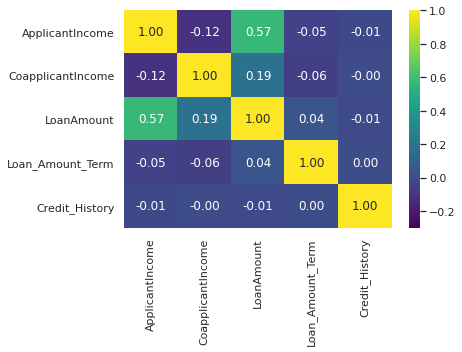
\includegraphics{notebook_files/notebook_18_0.png}
\caption{png}
\end{figure}

We also computed and plotted correlation matrix of features in the
dataset. There is only one pair of features, loan amount and applicant
income, which can be considered to be mildly positively correlated.
Other features, have nearly no correlation among them. This results is
quite suprising, as one would expect higher correlation of features.

\begin{Shaded}
\begin{Highlighting}[]
\NormalTok{sns.catplot(}\StringTok{"Loan_Status"}\NormalTok{, col}\OperatorTok{=}\StringTok{"Property_Area"}\NormalTok{, data}\OperatorTok{=}\NormalTok{dataset, kind}\OperatorTok{=}\StringTok{"count"}\NormalTok{)}
\NormalTok{sns.catplot(}\StringTok{"Loan_Status"}\NormalTok{, col}\OperatorTok{=}\StringTok{"Dependents"}\NormalTok{, data}\OperatorTok{=}\NormalTok{dataset, kind}\OperatorTok{=}\StringTok{"count"}\NormalTok{)}
\NormalTok{sns.catplot(}\StringTok{"Loan_Status"}\NormalTok{, col}\OperatorTok{=}\StringTok{"Gender"}\NormalTok{, data}\OperatorTok{=}\NormalTok{dataset, kind}\OperatorTok{=}\StringTok{"count"}\NormalTok{)}
\NormalTok{sns.catplot(}\StringTok{"Loan_Status"}\NormalTok{, col}\OperatorTok{=}\StringTok{"Married"}\NormalTok{, data}\OperatorTok{=}\NormalTok{dataset, kind}\OperatorTok{=}\StringTok{"count"}\NormalTok{)}
\NormalTok{sns.catplot(}\StringTok{"Loan_Status"}\NormalTok{, col}\OperatorTok{=}\StringTok{"Education"}\NormalTok{, data}\OperatorTok{=}\NormalTok{dataset, kind}\OperatorTok{=}\StringTok{"count"}\NormalTok{)}
\end{Highlighting}
\end{Shaded}

\textless{}seaborn.axisgrid.FacetGrid at 0x1ae6fca8ee0\textgreater{}

\begin{figure}
\centering
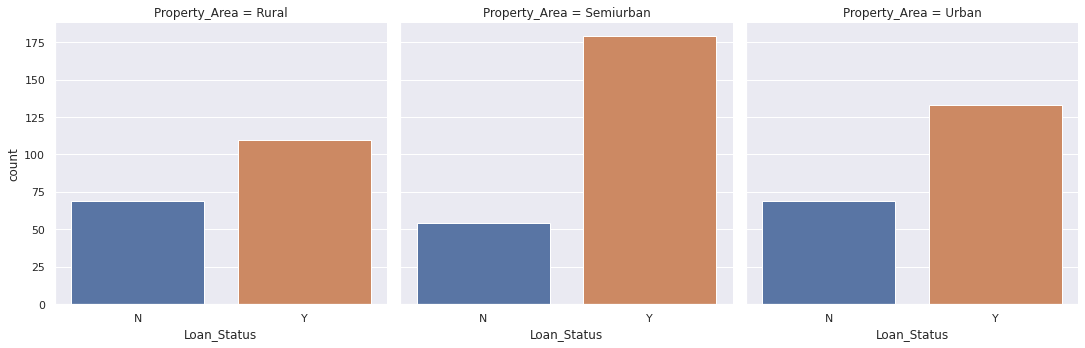
\includegraphics{notebook_files/notebook_20_1.png}
\caption{png}
\end{figure}

\begin{figure}
\centering
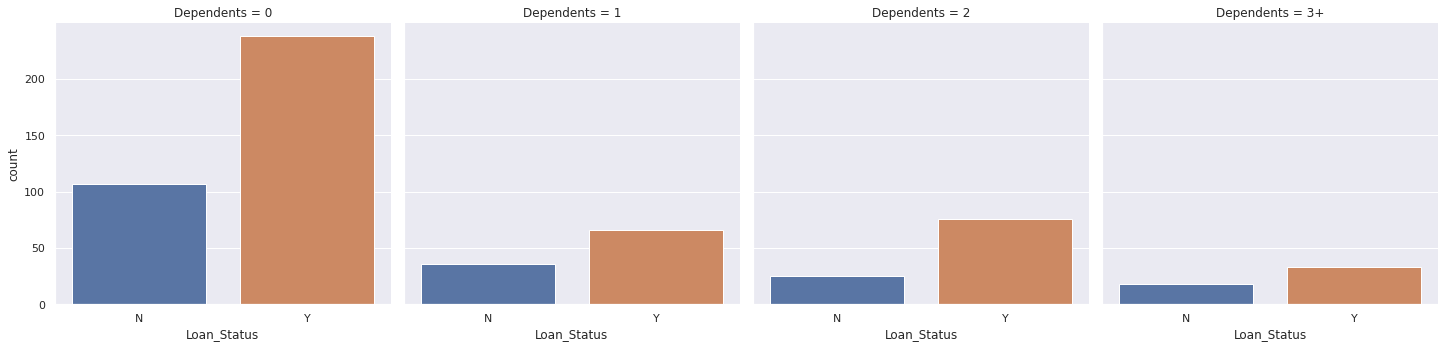
\includegraphics{notebook_files/notebook_20_2.png}
\caption{png}
\end{figure}

\begin{figure}
\centering
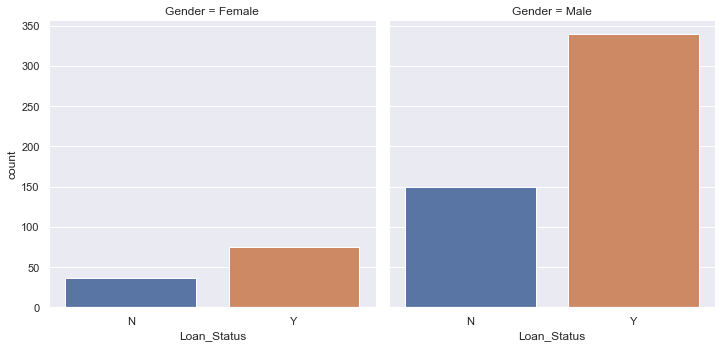
\includegraphics{notebook_files/notebook_20_3.png}
\caption{png}
\end{figure}

\begin{figure}
\centering
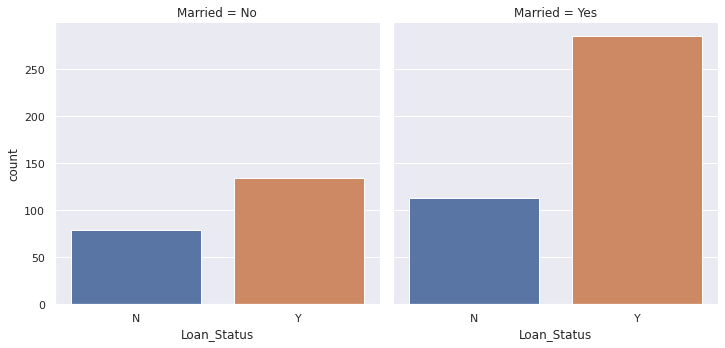
\includegraphics{notebook_files/notebook_20_4.png}
\caption{png}
\end{figure}

\begin{figure}
\centering
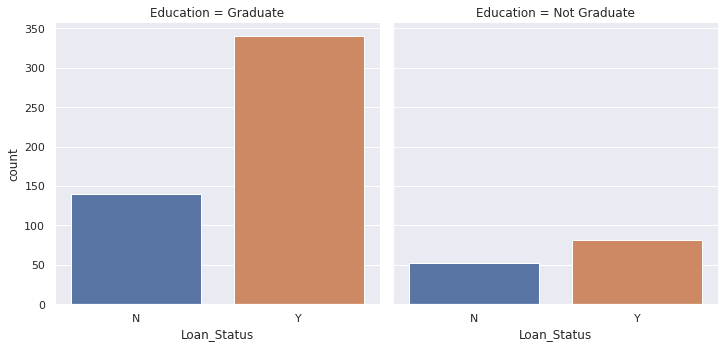
\includegraphics{notebook_files/notebook_20_5.png}
\caption{png}
\end{figure}

\begin{Shaded}
\begin{Highlighting}[]
\NormalTok{sns.countplot(X[}\StringTok{"Gender"}\NormalTok{])}
\NormalTok{plt.show()}
\NormalTok{sns.countplot(X[}\StringTok{"Married"}\NormalTok{])}
\NormalTok{plt.show()}
\NormalTok{sns.countplot(X[}\StringTok{"Dependents"}\NormalTok{])}
\NormalTok{plt.show()}
\NormalTok{sns.countplot(X[}\StringTok{"Education"}\NormalTok{])}
\NormalTok{plt.show()}
\NormalTok{sns.countplot(X[}\StringTok{"Self_Employed"}\NormalTok{])}
\NormalTok{plt.show()}
\NormalTok{sns.countplot(X[}\StringTok{"Property_Area"}\NormalTok{])}
\NormalTok{plt.show()}
\NormalTok{sns.distplot(X[}\StringTok{"ApplicantIncome"}\NormalTok{], kde}\OperatorTok{=}\VariableTok{True}\NormalTok{)}
\NormalTok{plt.show()}
\NormalTok{sns.distplot(X[}\StringTok{"CoapplicantIncome"}\NormalTok{], kde}\OperatorTok{=}\VariableTok{True}\NormalTok{)}
\NormalTok{plt.show()}
\NormalTok{sns.distplot(X[}\StringTok{"Credit_History"}\NormalTok{], kde}\OperatorTok{=}\VariableTok{True}\NormalTok{)}
\NormalTok{plt.show()}
\NormalTok{sns.distplot(X[}\StringTok{"LoanAmount"}\NormalTok{], kde}\OperatorTok{=}\VariableTok{True}\NormalTok{)}
\NormalTok{plt.show()}
\NormalTok{sns.distplot(X[}\StringTok{"Loan_Amount_Term"}\NormalTok{], kde}\OperatorTok{=}\VariableTok{True}\NormalTok{)}
\NormalTok{plt.show()}
\end{Highlighting}
\end{Shaded}

\begin{figure}
\centering
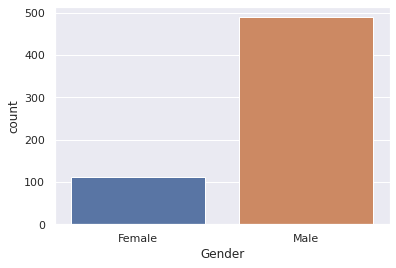
\includegraphics{notebook_files/notebook_21_0.png}
\caption{png}
\end{figure}

\begin{figure}
\centering
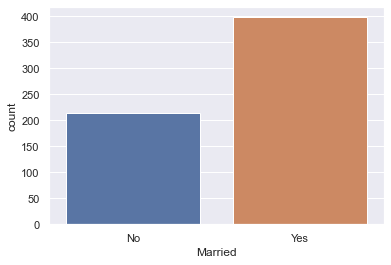
\includegraphics{notebook_files/notebook_21_1.png}
\caption{png}
\end{figure}

\begin{figure}
\centering
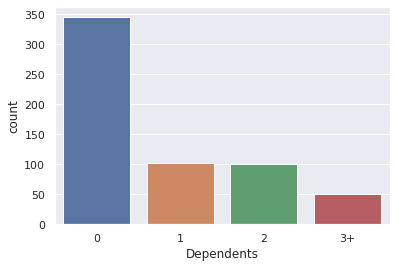
\includegraphics{notebook_files/notebook_21_2.png}
\caption{png}
\end{figure}

\begin{figure}
\centering
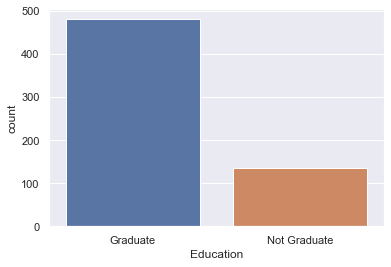
\includegraphics{notebook_files/notebook_21_3.png}
\caption{png}
\end{figure}

\begin{figure}
\centering
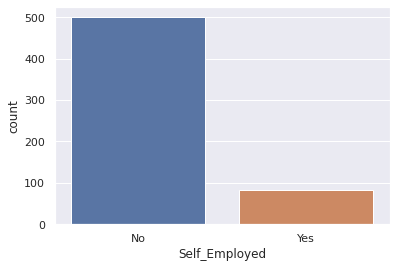
\includegraphics{notebook_files/notebook_21_4.png}
\caption{png}
\end{figure}

\begin{figure}
\centering
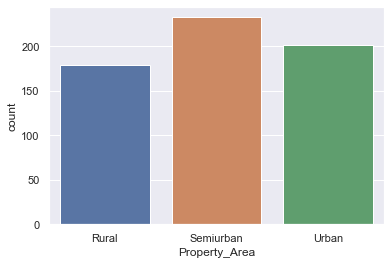
\includegraphics{notebook_files/notebook_21_5.png}
\caption{png}
\end{figure}

\begin{figure}
\centering
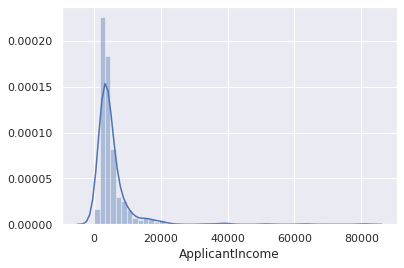
\includegraphics{notebook_files/notebook_21_6.png}
\caption{png}
\end{figure}

\begin{figure}
\centering
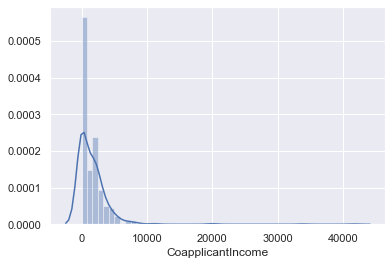
\includegraphics{notebook_files/notebook_21_7.png}
\caption{png}
\end{figure}

\begin{figure}
\centering
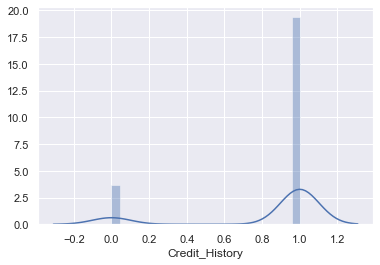
\includegraphics{notebook_files/notebook_21_8.png}
\caption{png}
\end{figure}

\begin{figure}
\centering
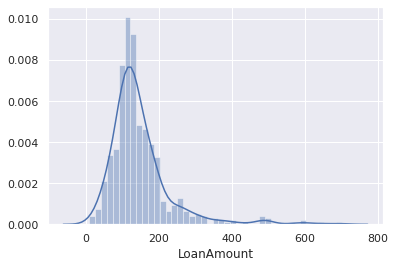
\includegraphics{notebook_files/notebook_21_9.png}
\caption{png}
\end{figure}

\begin{figure}
\centering
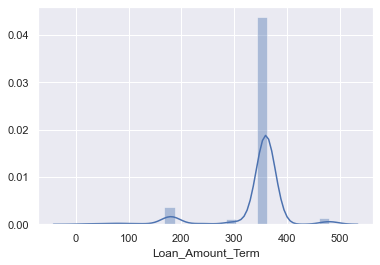
\includegraphics{notebook_files/notebook_21_10.png}
\caption{png}
\end{figure}

Most of the features are scattered along the x-axis. The only exception
is Loan Amount, which roughly follows the Chi-squared distribution.

\begin{Shaded}
\begin{Highlighting}[]
\NormalTok{sns.countplot(y)}
\end{Highlighting}
\end{Shaded}

\textless{}matplotlib.axes.\_subplots.AxesSubplot at
0x1ae6feb86a0\textgreater{}

\begin{figure}
\centering
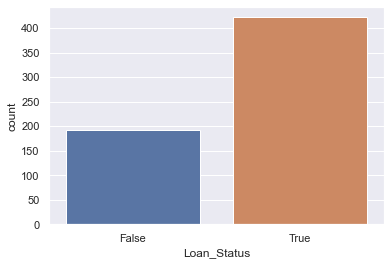
\includegraphics{notebook_files/notebook_23_1.png}
\caption{png}
\end{figure}

\begin{Shaded}
\begin{Highlighting}[]
\NormalTok{sns.pairplot(dataset, hue}\OperatorTok{=}\StringTok{"Loan_Status"}\NormalTok{, kind}\OperatorTok{=}\StringTok{"reg"}\NormalTok{, diag_kws}\OperatorTok{=}\NormalTok{\{}\StringTok{"alpha"}\NormalTok{: }\FloatTok{0.5}\NormalTok{\}, plot_kws}\OperatorTok{=}\NormalTok{\{}\StringTok{"scatter_kws"}\NormalTok{: \{}\StringTok{"alpha"}\NormalTok{: }\FloatTok{0.35}\NormalTok{\}\})}
\end{Highlighting}
\end{Shaded}

C:\Users\vojdo\Anaconda3\envs\ml\lib\site-packages\numpy\linalg\linalg.py:1965:
RuntimeWarning: invalid value encountered in greater large = s
\textgreater{} cutoff

\textless{}seaborn.axisgrid.PairGrid at 0x1ae6f9d7a90\textgreater{}

\begin{figure}
\centering
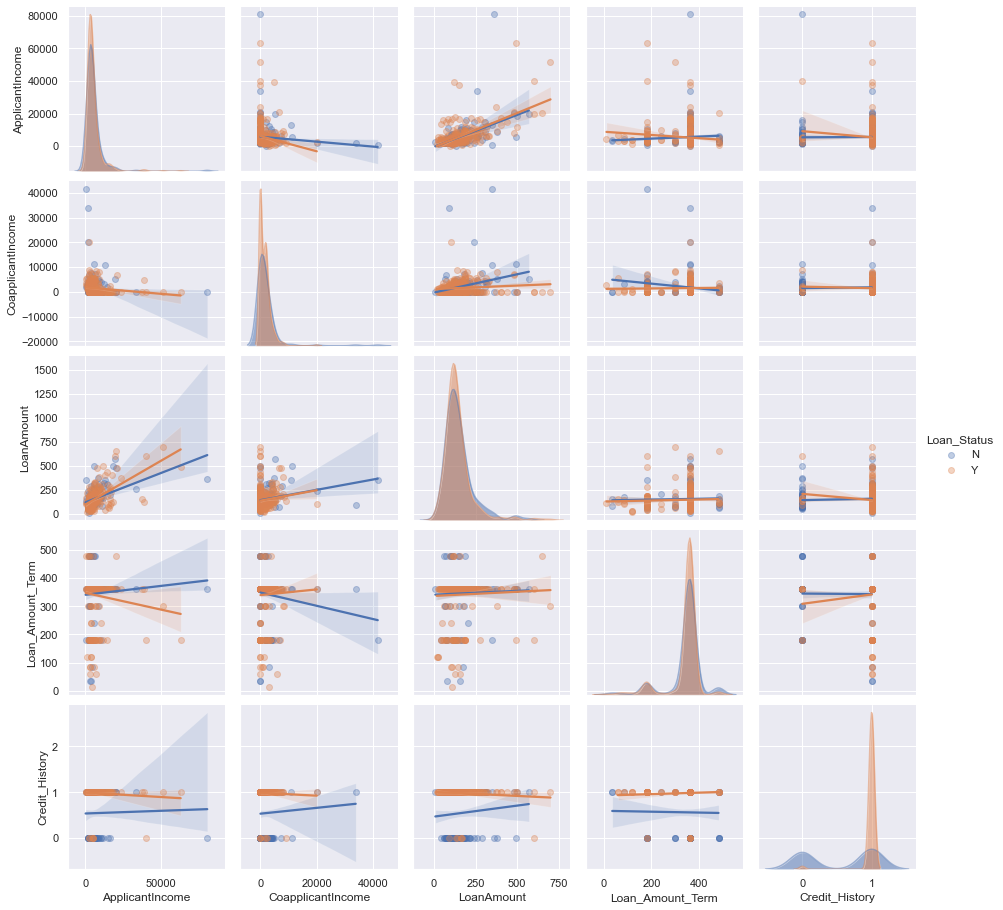
\includegraphics{notebook_files/notebook_24_2.png}
\caption{png}
\end{figure}

Credit history seems to have the highest impact on deciding whether the
loan should be approved or not. Clients with low credit score seem more
likely to be denied.

There are some cases where ApplicantIncome and CoapplicantIncome are
very low, their loan request gets approved, whereas in a few cases the
CoapplicantIncome is very high and ApplicantIncome is very low, the
request gets denied.

\hypertarget{data-preprocessing}{%
\subsection{2. Data preprocessing}\label{data-preprocessing}}

\begin{Shaded}
\begin{Highlighting}[]
\NormalTok{y.isna().}\BuiltInTok{sum}\NormalTok{()}
\end{Highlighting}
\end{Shaded}

0

Good, there are no N/A labels. We do not need to drop any rows. Besides
that, dropping a significant part of the dataset could have
misrepresenting effects.

Firstly, we will impute the missing values with \texttt{SimpleImputer}
and strategy \texttt{most\_frequent}. As \texttt{SimpleImputer} returns
an array, we will transform it back to a pandas dataframe. Another step
is encoding the categorical features using \texttt{OneHotEncoder}.
Lastly, we will scale the features with \texttt{StandardScaler}. Their
mean will therefore be 0 and variance 1.

The labels need significantly less preprocessing. Encoding their boolean
values is sufficient.

\begin{Shaded}
\begin{Highlighting}[]
\ImportTok{from}\NormalTok{ sklearn.preprocessing }\ImportTok{import}\NormalTok{ OrdinalEncoder, OneHotEncoder, StandardScaler}
\ImportTok{from}\NormalTok{ sklearn.pipeline }\ImportTok{import}\NormalTok{ make_pipeline}
\ImportTok{from}\NormalTok{ sklearn.compose }\ImportTok{import}\NormalTok{ make_column_transformer}
\ImportTok{from}\NormalTok{ sklearn.impute }\ImportTok{import}\NormalTok{ SimpleImputer}

\KeywordTok{class}\NormalTok{ NpToDf:}
\NormalTok{    columns }\OperatorTok{=}\NormalTok{ []}

    \KeywordTok{def} \FunctionTok{__init__}\NormalTok{(}\VariableTok{self}\NormalTok{, columns}\OperatorTok{=}\VariableTok{None}\NormalTok{):}
        \VariableTok{self}\NormalTok{.columns }\OperatorTok{=}\NormalTok{ columns}

    \KeywordTok{def}\NormalTok{ fit(}\VariableTok{self}\NormalTok{, X, }\OperatorTok{*}\NormalTok{args, }\OperatorTok{**}\NormalTok{kwargs):}
        \ControlFlowTok{return}\NormalTok{ X}

    \KeywordTok{def}\NormalTok{ fit_transform(}\VariableTok{self}\NormalTok{, X, }\OperatorTok{*}\NormalTok{args, }\OperatorTok{**}\NormalTok{kwargs):}
        \ControlFlowTok{return} \VariableTok{self}\NormalTok{.transform(X)}

    \KeywordTok{def}\NormalTok{ transform(}\VariableTok{self}\NormalTok{, X, }\OperatorTok{*}\NormalTok{args, }\OperatorTok{**}\NormalTok{kwargs):}
        \ControlFlowTok{return}\NormalTok{ pd.DataFrame(data}\OperatorTok{=}\NormalTok{X, columns}\OperatorTok{=}\VariableTok{self}\NormalTok{.columns)}

\NormalTok{pipe_X }\OperatorTok{=}\NormalTok{ make_pipeline(}
\NormalTok{    SimpleImputer(missing_values}\OperatorTok{=}\NormalTok{np.nan, strategy}\OperatorTok{=}\StringTok{"most_frequent"}\NormalTok{),}
\NormalTok{    NpToDf(X_train.columns),}
\NormalTok{    make_column_transformer(}
\NormalTok{        (OneHotEncoder(), [}\StringTok{'Gender'}\NormalTok{, }\StringTok{'Married'}\NormalTok{, }\StringTok{'Education'}\NormalTok{, }\StringTok{'Self_Employed'}\NormalTok{, }\StringTok{'Property_Area'}\NormalTok{, }\StringTok{'Dependents'}\NormalTok{]),}
\NormalTok{        remainder}\OperatorTok{=}\NormalTok{StandardScaler()),}
\NormalTok{    NpToDf(),}
\NormalTok{)}

\NormalTok{pipe_y }\OperatorTok{=}\NormalTok{ make_pipeline(}
\NormalTok{    OrdinalEncoder()}
\NormalTok{)}
\end{Highlighting}
\end{Shaded}

\begin{Shaded}
\begin{Highlighting}[]
\NormalTok{pipe_X.fit_transform(X_train)}
\NormalTok{train_X }\OperatorTok{=}\NormalTok{ pipe_X.transform(X_train)}
\NormalTok{test_X }\OperatorTok{=}\NormalTok{ pipe_X.transform(X_test)}

\NormalTok{train_y }\OperatorTok{=}\NormalTok{ pipe_y.fit_transform(y_train.to_numpy().reshape(}\OperatorTok{-}\DecValTok{1}\NormalTok{, }\DecValTok{1}\NormalTok{)).reshape(}\OperatorTok{-}\DecValTok{1}\NormalTok{)}
\NormalTok{test_y }\OperatorTok{=}\NormalTok{ pipe_y.fit_transform(y_test.to_numpy().reshape(}\OperatorTok{-}\DecValTok{1}\NormalTok{, }\DecValTok{1}\NormalTok{)).reshape(}\OperatorTok{-}\DecValTok{1}\NormalTok{)}
\end{Highlighting}
\end{Shaded}

Some helper functions for training and evaluation of our models.

\begin{Shaded}
\begin{Highlighting}[]
\ImportTok{from}\NormalTok{ sklearn.metrics }\ImportTok{import}\NormalTok{ mean_squared_error, f1_score}
\ImportTok{from}\NormalTok{ sklearn.model_selection }\ImportTok{import}\NormalTok{ cross_val_score}
\ImportTok{import}\NormalTok{ matplotlib.pyplot }\ImportTok{as}\NormalTok{ plt}

\KeywordTok{def}\NormalTok{ evaluate(clf, X_test, y_test):}
\NormalTok{    y_pred }\OperatorTok{=}\NormalTok{ clf.predict(X_test)}
\NormalTok{    scores }\OperatorTok{=}\NormalTok{ cross_val_score(clf, X_test, y_test, cv}\OperatorTok{=}\DecValTok{10}\NormalTok{)}

    \BuiltInTok{print}\NormalTok{(}\SpecialStringTok{f"RMSE: }\SpecialCharTok{\{}\NormalTok{mean_squared_error(y_test, y_pred, squared }\OperatorTok{=} \VariableTok{False}\NormalTok{)}\SpecialCharTok{:.4f\}}\SpecialStringTok{"}\NormalTok{)   }
    \BuiltInTok{print}\NormalTok{(}\SpecialStringTok{f"Accuracy: }\SpecialCharTok{\{}\NormalTok{scores}\SpecialCharTok{.}\NormalTok{mean()}\SpecialCharTok{:.3f\}}\SpecialStringTok{ ± }\SpecialCharTok{\{}\NormalTok{scores}\SpecialCharTok{.}\NormalTok{std() }\OperatorTok{*} \DecValTok{2}\SpecialCharTok{:.3f\}}\SpecialStringTok{"}\NormalTok{)}
    \BuiltInTok{print}\NormalTok{(}\StringTok{"F1 Score: }\SpecialCharTok\NormalTok{ f1_score(y_test, y_pred, average}\OperatorTok{=}\StringTok{'weighted'}\NormalTok{))}
\end{Highlighting}
\end{Shaded}

\begin{Shaded}
\begin{Highlighting}[]
\ImportTok{from}\NormalTok{ sklearn.metrics }\ImportTok{import}\NormalTok{ plot_roc_curve}

\KeywordTok{def}\NormalTok{ roc(clf, test_X, test_y):}
\NormalTok{    plot_roc_curve(clf, test_X, test_y)}
\NormalTok{    plt.plot([}\DecValTok{0}\NormalTok{, }\DecValTok{1}\NormalTok{], [}\DecValTok{0}\NormalTok{, }\DecValTok{1}\NormalTok{], linestyle}\OperatorTok{=}\StringTok{'--'}\NormalTok{, lw}\OperatorTok{=}\DecValTok{2}\NormalTok{, color}\OperatorTok{=}\StringTok{'r'}\NormalTok{, label}\OperatorTok{=}\StringTok{'Chance'}\NormalTok{, alpha}\OperatorTok{=}\NormalTok{.}\DecValTok{8}\NormalTok{)}
\NormalTok{    plt.legend()}
\end{Highlighting}
\end{Shaded}

\begin{Shaded}
\begin{Highlighting}[]
\ImportTok{from}\NormalTok{ sklearn.metrics }\ImportTok{import}\NormalTok{ plot_precision_recall_curve }\ImportTok{as}\NormalTok{ prc}
\ImportTok{from}\NormalTok{ sklearn.metrics }\ImportTok{import}\NormalTok{ precision_recall_curve}
\end{Highlighting}
\end{Shaded}

\begin{Shaded}
\begin{Highlighting}[]
\ImportTok{from}\NormalTok{ sklearn.metrics }\ImportTok{import}\NormalTok{ plot_confusion_matrix}
\ImportTok{from}\NormalTok{ sklearn.metrics }\ImportTok{import}\NormalTok{ confusion_matrix}
\ImportTok{from}\NormalTok{ sklearn.model_selection }\ImportTok{import}\NormalTok{ GridSearchCV}

\KeywordTok{def}\NormalTok{ confusion(clf, X_test, y_test):}
\NormalTok{    plot_confusion_matrix(clf, X_test, y_test, cmap}\OperatorTok{=}\NormalTok{plt.cm.Blues)    }
                        
\end{Highlighting}
\end{Shaded}

\begin{Shaded}
\begin{Highlighting}[]
\KeywordTok{def}\NormalTok{ get_gscv(clf, param_grid, verbose}\OperatorTok{=}\DecValTok{1}\NormalTok{, }\OperatorTok{**}\NormalTok{kwargs):}
\NormalTok{    gs }\OperatorTok{=}\NormalTok{ GridSearchCV(clf, param_grid, verbose}\OperatorTok{=}\NormalTok{verbose, cv}\OperatorTok{=}\NormalTok{kwargs.get(}\StringTok{"cv"}\NormalTok{, }\DecValTok{3}\NormalTok{), n_jobs}\OperatorTok{=}\NormalTok{kwargs.get(}\StringTok{"workers"}\NormalTok{, }\DecValTok{-2}\NormalTok{))}
\NormalTok{    gs.fit(train_X, train_y, }\OperatorTok{**}\NormalTok{kwargs)}
\NormalTok{    score }\OperatorTok{=}\NormalTok{ gs.score(test_X, test_y)}
    \BuiltInTok{print}\NormalTok{(}\SpecialStringTok{f"Best parameters: }\SpecialCharTok{\{gs.}\NormalTok{best_params_}\SpecialCharTok{\}}\SpecialStringTok{, with F1 score of }\SpecialCharTok{\{}\NormalTok{score}\SpecialCharTok{:.2f\}}\SpecialStringTok{"}\NormalTok{)}
    \ControlFlowTok{return}\NormalTok{ gs.best_estimator_}
\end{Highlighting}
\end{Shaded}

In the following 4 sections, we will always start by running a grid
search tuning hyperparameters of our models. There is a wrapper for
keras sequential models, which we will use for grid searching. All
models will be trained on the same training set. We chose these
evaluation metrics - \textbf{RMSE} - measures error of the predictions
compared to actual values, the lower the better. - \textbf{Acurracy}
computed with cross validation score - is the proportion of correct
predictions (both true positives and true negatives) among the total
number of cases examined, the higher the better - \textbf{F1 score} - is
weighted average of precision and recall, the best value is 1, the worst
is 0 - \textbf{Receiver Operating Characteristic curve} - measures the
ability of a model to distinguish between classes - \textbf{Precision
Recall curve} - shows the tradeoff between precision and recall for
different threshold - \textbf{Confusion matrix} - shows the number of
True Positive (TP), False Negative (FN), True Negative (TN), False
Positive (FP) classifications.

\hypertarget{naive-baseline-model}{%
\subsection{3. Naive baseline model}\label{naive-baseline-model}}

This is a simple classifier, which chooses the class based on training
set class distribution.

It is very basic and is affected by the chosen train/test split a lot.

\begin{Shaded}
\begin{Highlighting}[]
\ImportTok{from}\NormalTok{ sklearn.dummy }\ImportTok{import}\NormalTok{ DummyClassifier}

\NormalTok{dummy_clf }\OperatorTok{=}\NormalTok{ DummyClassifier(strategy}\OperatorTok{=}\StringTok{"stratified"}\NormalTok{)}

\NormalTok{dummy_clf.fit(train_X, train_y)}

\NormalTok{evaluate(dummy_clf, test_X, test_y)}
\NormalTok{roc(dummy_clf, test_X, test_y)}
\NormalTok{prc(dummy_clf, test_X, test_y)}
\NormalTok{confusion(dummy_clf, test_X, test_y)}
\NormalTok{plt.show()}
\end{Highlighting}
\end{Shaded}

RMSE: 0.6502 Accuracy: 0.538 ± 0.158 F1 Score: 0.58

\begin{figure}
\centering
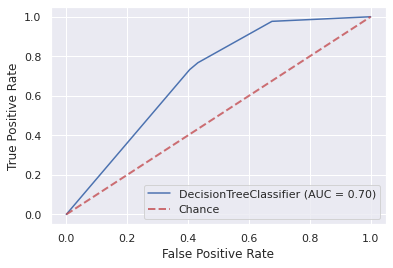
\includegraphics{notebook_files/notebook_41_1.png}
\caption{png}
\end{figure}

\begin{figure}
\centering
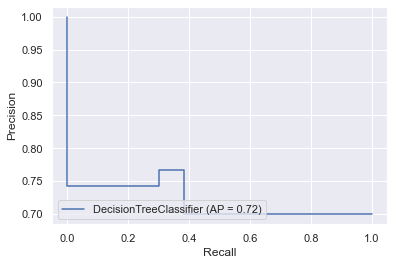
\includegraphics{notebook_files/notebook_41_2.png}
\caption{png}
\end{figure}

\begin{figure}
\centering
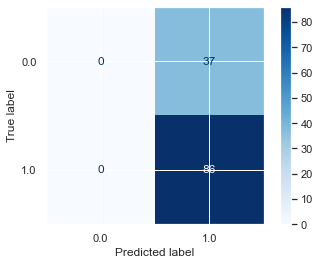
\includegraphics{notebook_files/notebook_41_3.png}
\caption{png}
\end{figure}

\hypertarget{decision-tree-classifier}{%
\subsection{4. Decision tree
classifier}\label{decision-tree-classifier}}

Decision trees are among the most used classification models. They
iteratively split the dataset, until a tree conforming to given
parameters has been constructed. In leaves they contain class labels.
Internal nodes represent kind of a boolean test, usually a value of a
sample's feature, according to which the algorithm chooses the
respective edge on the way to leaves. The tests can also use entropy and
information gain to choose the best edge. There are many to ways to
construct a tree, therefore extensive hyperparameter tunning is
suitable. Decision trees can also be pruned, etheir during construction
of after it.

\begin{Shaded}
\begin{Highlighting}[]
\ImportTok{from}\NormalTok{ sklearn.tree }\ImportTok{import}\NormalTok{ DecisionTreeClassifier}

\NormalTok{dtree_clf }\OperatorTok{=}\NormalTok{ DecisionTreeClassifier()}
\NormalTok{dtree_values }\OperatorTok{=}\NormalTok{ \{}\StringTok{"criterion"}\NormalTok{: [}\StringTok{"gini"}\NormalTok{, }\StringTok{"entropy"}\NormalTok{],}
                \StringTok{"max_depth"}\NormalTok{: [}\DecValTok{1}\NormalTok{, }\DecValTok{2}\NormalTok{, }\DecValTok{5}\NormalTok{, }\DecValTok{10}\NormalTok{, }\DecValTok{16}\NormalTok{, }\VariableTok{None}\NormalTok{],}
                \StringTok{"max_leaf_nodes"}\NormalTok{: [}\DecValTok{6}\NormalTok{, }\DecValTok{8}\NormalTok{, }\DecValTok{10}\NormalTok{, }\DecValTok{12}\NormalTok{, }\DecValTok{20}\NormalTok{, }\VariableTok{None}\NormalTok{],}
                \StringTok{"max_features"}\NormalTok{: [}\StringTok{"auto"}\NormalTok{, }\StringTok{"sqrt"}\NormalTok{, }\StringTok{"log2"}\NormalTok{, }\DecValTok{2}\NormalTok{, }\DecValTok{4}\NormalTok{, }\DecValTok{8}\NormalTok{]\}}
                
\NormalTok{tree_clf }\OperatorTok{=}\NormalTok{ get_gscv(dtree_clf, dtree_values)}
\end{Highlighting}
\end{Shaded}

Fitting 3 folds for each of 432 candidates, totalling 1296 fits

Best parameters: \{`criterion': `gini', `max\_depth': 1,
`max\_features': 8, `max\_leaf\_nodes': 6\}, with F1 score of 0.80

\begin{Shaded}
\begin{Highlighting}[]
\NormalTok{evaluate(tree_clf, test_X, test_y)}
\NormalTok{roc(tree_clf, test_X, test_y)}
\NormalTok{prc(tree_clf, test_X, test_y)}
\NormalTok{confusion(tree_clf, test_X, test_y)}
\NormalTok{plt.show()}
\end{Highlighting}
\end{Shaded}

RMSE: 0.4508 Accuracy: 0.716 ± 0.147 F1 Score: 0.77

\begin{figure}
\centering
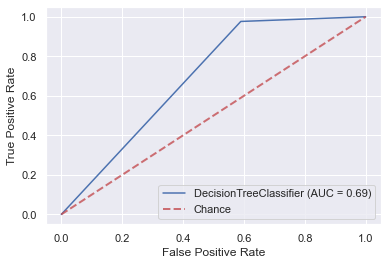
\includegraphics{notebook_files/notebook_44_1.png}
\caption{png}
\end{figure}

\begin{figure}
\centering
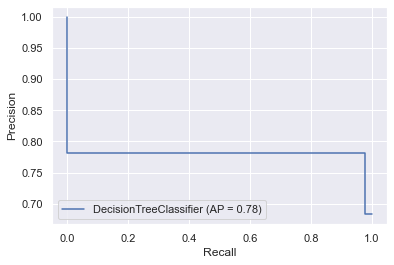
\includegraphics{notebook_files/notebook_44_2.png}
\caption{png}
\end{figure}

\begin{figure}
\centering
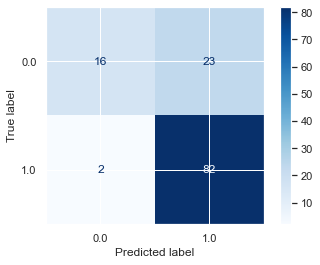
\includegraphics{notebook_files/notebook_44_3.png}
\caption{png}
\end{figure}

\hypertarget{knn-classifier}{%
\subsection{5. KNN classifier}\label{knn-classifier}}

Another popular classification algorithm, an example of instace-based
learning or lazy learning. This time, all distances from a data point to
other points are computed, and k-closest neighbours are chosen. Then,
the class memberships of the \emph{k-closest} members are considered,
with the original data point taking a class label from the most occuring
one among its \emph{k-closest} neighbours. For the distance metrics,
\emph{Euclidean} or \emph{Hamming} distances are usually used. There is
a tradeoff in the number of \emph{k-closest} neighbours. Smaller
\emph{k}, signifies the result of noise on classification, but makes the
various classses more distinct and vice versa with higher \emph{k}.

\begin{Shaded}
\begin{Highlighting}[]
\ImportTok{from}\NormalTok{ sklearn.neighbors }\ImportTok{import}\NormalTok{ KNeighborsClassifier}

\NormalTok{knn_clf }\OperatorTok{=}\NormalTok{ KNeighborsClassifier()}
\NormalTok{knn_values }\OperatorTok{=}\NormalTok{ \{}\StringTok{"n_neighbors"}\NormalTok{: }\BuiltInTok{list}\NormalTok{(}\BuiltInTok{range}\NormalTok{(}\DecValTok{2}\NormalTok{, }\DecValTok{16}\NormalTok{, }\DecValTok{2}\NormalTok{)), }
              \StringTok{"algorithm"}\NormalTok{: [}\StringTok{"auto"}\NormalTok{, }\StringTok{"ball_tree"}\NormalTok{, }\StringTok{"kd_tree"}\NormalTok{, }\StringTok{"brute"}\NormalTok{],}
              \StringTok{"leaf_size"}\NormalTok{: [}\DecValTok{10}\NormalTok{, }\DecValTok{20}\NormalTok{, }\DecValTok{30}\NormalTok{, }\DecValTok{40}\NormalTok{, }\DecValTok{50}\NormalTok{], }
              \StringTok{"p"}\NormalTok{: [}\DecValTok{1}\NormalTok{, }\DecValTok{2}\NormalTok{], }
              \StringTok{"weights"}\NormalTok{: [}\StringTok{"uniform"}\NormalTok{, }\StringTok{"distance"}\NormalTok{]\}}
              
\NormalTok{knn_clf }\OperatorTok{=}\NormalTok{ get_gscv(knn_clf, knn_values)}
\end{Highlighting}
\end{Shaded}

Fitting 3 folds for each of 560 candidates, totalling 1680 fits

Best parameters: \{`algorithm': `auto', `leaf\_size': 10,
`n\_neighbors': 12, `p': 2, `weights': `uniform'\}, with F1 score of
0.80

\begin{Shaded}
\begin{Highlighting}[]
\NormalTok{evaluate(knn_clf, test_X, test_y)}
\NormalTok{roc(knn_clf, test_X, test_y)}
\NormalTok{prc(knn_clf, test_X, test_y)}
\NormalTok{confusion(knn_clf, test_X, test_y)}
\NormalTok{plt.show()}
\end{Highlighting}
\end{Shaded}

RMSE: 0.4508 Accuracy: 0.797 ± 0.234 F1 Score: 0.78

\begin{figure}
\centering
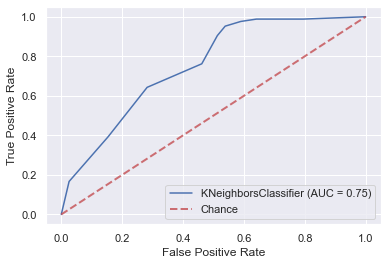
\includegraphics{notebook_files/notebook_48_1.png}
\caption{png}
\end{figure}

\begin{figure}
\centering
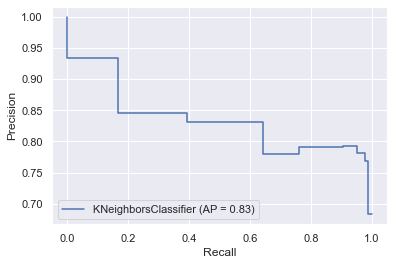
\includegraphics{notebook_files/notebook_48_2.png}
\caption{png}
\end{figure}

\begin{figure}
\centering
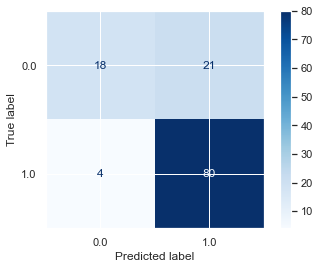
\includegraphics{notebook_files/notebook_48_3.png}
\caption{png}
\end{figure}

\hypertarget{support-vector-machine}{%
\subsection{6. Support Vector Machine}\label{support-vector-machine}}

Support Vector Machines, abbr. SVM, is a supervised-learning algorithm
used mainly for binary classification, although it is possible to use
for multi-class classification by combing several SVMs. It creates
hyperplanes in a multi-dimensional feature space, which are then used
for generalization and classifications of data points. The best
performing hyperplanes are those having the biggest maximum margin,
i.e.~the closest data points from both classes are as far as possible.
In order to transform input data into a desired form, SVM uses so called
kernel functions, which return the inner product between two points in a
suitable feature space.

\begin{Shaded}
\begin{Highlighting}[]
\ImportTok{from}\NormalTok{ sklearn.svm }\ImportTok{import}\NormalTok{ SVC}

\NormalTok{svc_clf }\OperatorTok{=}\NormalTok{ SVC()}
\NormalTok{svc_values }\OperatorTok{=}\NormalTok{ \{}\StringTok{"C"}\NormalTok{: [.}\DecValTok{8}\NormalTok{, }\FloatTok{1.0}\NormalTok{, }\FloatTok{1.2}\NormalTok{, }\FloatTok{1.5}\NormalTok{, }\FloatTok{2.0}\NormalTok{],}
              \StringTok{"kernel"}\NormalTok{: [}\StringTok{"linear"}\NormalTok{,}\StringTok{"poly"}\NormalTok{,}\StringTok{"rbf"}\NormalTok{,}\StringTok{"sigmoid"}\NormalTok{],}
              \StringTok{"degree"}\NormalTok{: [}\DecValTok{2}\NormalTok{, }\DecValTok{3}\NormalTok{, }\DecValTok{4}\NormalTok{, }\DecValTok{5}\NormalTok{], }
              \StringTok{"gamma"}\NormalTok{: [}\StringTok{"scale"}\NormalTok{, }\StringTok{"auto"}\NormalTok{], }
              \StringTok{"coef0"}\NormalTok{: [.}\DecValTok{0}\NormalTok{, }\FloatTok{.5}\NormalTok{, }\FloatTok{1.0}\NormalTok{, }\FloatTok{1.5}\NormalTok{]\}}
              
\NormalTok{svm_clf }\OperatorTok{=}\NormalTok{ get_gscv(svc_clf, svc_values)}
\end{Highlighting}
\end{Shaded}

Fitting 3 folds for each of 640 candidates, totalling 1920 fits

Best parameters: \{`C': 0.8, `coef0': 0.0, `degree': 2, `gamma': `auto',
`kernel': `poly'\}, with F1 score of 0.80

\begin{Shaded}
\begin{Highlighting}[]
\NormalTok{evaluate(svm_clf, test_X, test_y)}
\NormalTok{roc(svm_clf, test_X, test_y)}
\NormalTok{prc(svm_clf, test_X, test_y)}
\NormalTok{confusion(svm_clf, test_X, test_y)}
\NormalTok{plt.show()}
\end{Highlighting}
\end{Shaded}

RMSE: 0.4508 Accuracy: 0.796 ± 0.213 F1 Score: 0.77

\begin{figure}
\centering
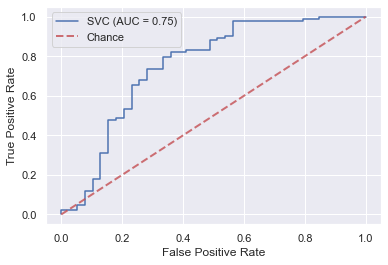
\includegraphics{notebook_files/notebook_52_1.png}
\caption{png}
\end{figure}

\begin{figure}
\centering
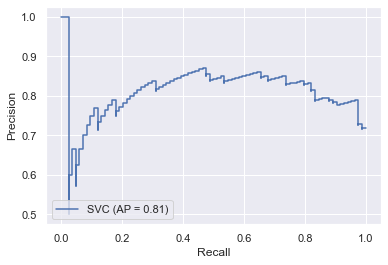
\includegraphics{notebook_files/notebook_52_2.png}
\caption{png}
\end{figure}

\begin{figure}
\centering
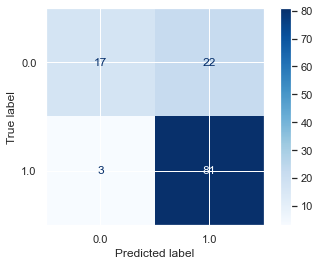
\includegraphics{notebook_files/notebook_52_3.png}
\caption{png}
\end{figure}

\hypertarget{deep-neural-network}{%
\subsection{7. Deep Neural Network}\label{deep-neural-network}}

Deep neural networks (DNNs) are artifical neural (ANNs) networks with
several hidden layers. Each layer is a fixed number of artificial
neurons, which accept an input, process it, and send it to the next
layer. The layers are organized followingly:

input layer → hidden layers → output layer.

Each layer has an activation function, whose choice greatly influences
the overall performance. In classification tasks, the output layer
yields the final class labels. We will use \texttt{Sequential\ model}
from \texttt{Keras} as our DNN.

For the activation functions we will stick with ReLU or Recrified Linear
Units. These are nearly linear functions commonly used in DNNs and
provide the best results. Leaky ReLU may be used as well.

We will be choosing either Adam, Stochastic Gradient Descent or RMSProp
optimizer.

Batch size will remain constant 32 and epochs 10-15, since these numbers
offer the best results for the time spent learning.

We have experimented with dropout a bit, but found little to no
difference when using it, so it will be kept at 0

\begin{Shaded}
\begin{Highlighting}[]
\ImportTok{import}\NormalTok{ tensorflow }\ImportTok{as}\NormalTok{ tf}
\ImportTok{import}\NormalTok{ itertools}
\ImportTok{import}\NormalTok{ itertools}
\ImportTok{import}\NormalTok{ gc}

\ImportTok{import}\NormalTok{ keras.backend }\ImportTok{as}\NormalTok{ K}
\ImportTok{from}\NormalTok{ keras.optimizers }\ImportTok{import}\NormalTok{ Adam, SGD, RMSprop}
\ImportTok{from}\NormalTok{ keras.models }\ImportTok{import}\NormalTok{ Sequential}
\ImportTok{from}\NormalTok{ keras.callbacks }\ImportTok{import}\NormalTok{ EarlyStopping}
\ImportTok{from}\NormalTok{ keras.layers }\ImportTok{import}\NormalTok{ Dense, Dropout}
\ImportTok{from}\NormalTok{ sklearn.metrics }\ImportTok{import}\NormalTok{ classification_report, confusion_matrix}
\ImportTok{from}\NormalTok{ keras.wrappers.scikit_learn }\ImportTok{import}\NormalTok{ KerasClassifier}
\end{Highlighting}
\end{Shaded}

Using TensorFlow backend.

\begin{Shaded}
\begin{Highlighting}[]
\NormalTok{layer_sizes }\OperatorTok{=}\NormalTok{ [[[}\DecValTok{8}\NormalTok{, }\DecValTok{16}\NormalTok{, }\DecValTok{32}\NormalTok{, }\DecValTok{64}\NormalTok{] }\ControlFlowTok{for}\NormalTok{ _ }\KeywordTok{in} \BuiltInTok{range}\NormalTok{(size)] }\ControlFlowTok{for}\NormalTok{ size }\KeywordTok{in} \BuiltInTok{range}\NormalTok{(}\DecValTok{6}\NormalTok{, }\DecValTok{7}\NormalTok{)]}
\NormalTok{layer_combinations }\OperatorTok{=} \BuiltInTok{list}\NormalTok{(itertools.chain.from_iterable(}\BuiltInTok{map}\NormalTok{(}\KeywordTok{lambda}\NormalTok{ sublist: }\BuiltInTok{list}\NormalTok{(itertools.product(}\OperatorTok{*}\NormalTok{sublist)), layer_sizes)))}
\KeywordTok{del}\NormalTok{ layer_sizes}

\NormalTok{gc.collect()}
\NormalTok{gc.enable()}
\end{Highlighting}
\end{Shaded}

\begin{Shaded}
\begin{Highlighting}[]
\KeywordTok{def}\NormalTok{ build_net(optim, layers, lr, dropout, }\OperatorTok{**}\NormalTok{kwargs):}
\NormalTok{    K.clear_session()}
\NormalTok{    model }\OperatorTok{=}\NormalTok{ Sequential()}
\NormalTok{    model.add(Dense(layers[}\DecValTok{0}\NormalTok{], input_shape}\OperatorTok{=}\NormalTok{(train_X.shape[}\DecValTok{1}\NormalTok{],), activation}\OperatorTok{=}\StringTok{'relu'}\NormalTok{))}
\NormalTok{    model.add(Dropout(dropout))}
    \ControlFlowTok{for}\NormalTok{ layer }\KeywordTok{in}\NormalTok{ layers[}\DecValTok{1}\NormalTok{:]:}
\NormalTok{        model.add(Dense(layer, activation}\OperatorTok{=}\StringTok{'relu'}\NormalTok{))}
\NormalTok{        model.add(Dropout(dropout))}
\NormalTok{    model.add(Dense(}\DecValTok{2}\NormalTok{, activation}\OperatorTok{=}\StringTok{'softmax'}\NormalTok{))}
\NormalTok{    model.}\BuiltInTok{compile}\NormalTok{(loss}\OperatorTok{=}\StringTok{'categorical_crossentropy'}\NormalTok{, optimizer}\OperatorTok{=}\NormalTok{optim(learning_rate}\OperatorTok{=}\NormalTok{lr), metrics}\OperatorTok{=}\NormalTok{[}\StringTok{'accuracy'}\NormalTok{]) }
    \ControlFlowTok{return}\NormalTok{ model}
\end{Highlighting}
\end{Shaded}

\begin{Shaded}
\begin{Highlighting}[]
\NormalTok{net_clf }\OperatorTok{=}\NormalTok{ KerasClassifier(build_fn}\OperatorTok{=}\NormalTok{build_net, verbose}\OperatorTok{=}\DecValTok{0}\NormalTok{)}

\NormalTok{layer_sizes }\OperatorTok{=}\NormalTok{ [[[}\DecValTok{32}\NormalTok{, }\DecValTok{64}\NormalTok{, }\DecValTok{128}\NormalTok{] }\ControlFlowTok{for}\NormalTok{ _ }\KeywordTok{in} \BuiltInTok{range}\NormalTok{(size)] }\ControlFlowTok{for}\NormalTok{ size }\KeywordTok{in} \BuiltInTok{range}\NormalTok{(}\DecValTok{3}\NormalTok{, }\DecValTok{5}\NormalTok{)]}
\NormalTok{layer_combinations }\OperatorTok{=} \BuiltInTok{list}\NormalTok{(itertools.chain.from_iterable(}\BuiltInTok{map}\NormalTok{(}\KeywordTok{lambda}\NormalTok{ sublist: }\BuiltInTok{list}\NormalTok{(itertools.product(}\OperatorTok{*}\NormalTok{sublist)), layer_sizes)))}

\NormalTok{net_values }\OperatorTok{=}\NormalTok{ \{}\StringTok{"optim"}\NormalTok{: [Adam, SGD, RMSprop], }\StringTok{"epochs"}\NormalTok{: [}\DecValTok{10}\NormalTok{], }\StringTok{"batch_size"}\NormalTok{: [}\DecValTok{32}\NormalTok{], }\StringTok{"layers"}\NormalTok{: layer_combinations, }\StringTok{"dropout"}\NormalTok{: [.}\DecValTok{1}\NormalTok{], }\StringTok{"lr"}\NormalTok{: [}\FloatTok{4e-3}\NormalTok{, }\FloatTok{1e-4}\NormalTok{]\}}

\NormalTok{es }\OperatorTok{=}\NormalTok{ EarlyStopping(monitor}\OperatorTok{=}\StringTok{'loss'}\NormalTok{, min_delta}\OperatorTok{=}\DecValTok{0}\NormalTok{, patience}\OperatorTok{=}\DecValTok{2}\NormalTok{, verbose}\OperatorTok{=}\DecValTok{0}\NormalTok{, mode}\OperatorTok{=}\StringTok{'auto'}\NormalTok{)}

\NormalTok{dnn_clf }\OperatorTok{=}\NormalTok{ get_gscv(net_clf, net_values, callbacks}\OperatorTok{=}\NormalTok{[es])}
\end{Highlighting}
\end{Shaded}

Fitting 3 folds for each of 2880 candidates, totalling 8640 fits

\hypertarget{best-parameters-batch_size-32-dropout-0.1-epochs-10-layers-32-64-32-64-lr-0.004-optim-class-keras.optimizers.rmsprop-with-f1-score-of-0.78}{%
\subparagraph{1. Best parameters: \{`batch\_size': 32, `dropout': 0.1,
`epochs': 10, `layers': (32, 64, 32, 64), `lr': 0.004, `optim':
\textless{}class `keras.optimizers.RMSprop'\textgreater{}\}, with F1
score of
0.78}\label{best-parameters-batch_size-32-dropout-0.1-epochs-10-layers-32-64-32-64-lr-0.004-optim-class-keras.optimizers.rmsprop-with-f1-score-of-0.78}}

\hypertarget{best-parameters-batch_size-32-dropout-0.0-epochs-15-layers-8-32-8-32-lr-0.001-optim-class-keras.optimizers.rmsprop-with-f1-score-of-0.77}{%
\subparagraph{2. Best parameters: \{`batch\_size': 32, `dropout': 0.0,
`epochs': 15, `layers': (8, 32, 8, 32), `lr': 0.001, `optim':
\textless{}class `keras.optimizers.RMSprop'\textgreater{}\}, with F1
score of
0.77}\label{best-parameters-batch_size-32-dropout-0.0-epochs-15-layers-8-32-8-32-lr-0.001-optim-class-keras.optimizers.rmsprop-with-f1-score-of-0.77}}

\hypertarget{best-parameters-batch_size-32-dropout-0.1-epochs-12-layers-64-64-64-64-32-16-lr-0.0003-optim-class-keras.optimizers.adam-with-f1-score-of-0.85}{%
\subparagraph{3. Best parameters: \{`batch\_size': 32, `dropout': 0.1,
`epochs': 12, `layers': (64, 64, 64, 64, 32, 16), `lr': 0.0003, `optim':
\textless{}class `keras.optimizers.Adam'\textgreater{}\}, with F1 score
of
0.85}\label{best-parameters-batch_size-32-dropout-0.1-epochs-12-layers-64-64-64-64-32-16-lr-0.0003-optim-class-keras.optimizers.adam-with-f1-score-of-0.85}}

\begin{Shaded}
\begin{Highlighting}[]
\NormalTok{ohe }\OperatorTok{=}\NormalTok{ OneHotEncoder()}

\NormalTok{nn_train_y }\OperatorTok{=}\NormalTok{ ohe.fit_transform(y_train.to_numpy().reshape(}\OperatorTok{-}\DecValTok{1}\NormalTok{, }\DecValTok{1}\NormalTok{))}
\NormalTok{nn_test_y }\OperatorTok{=}\NormalTok{ ohe.transform(y_test.to_numpy().reshape(}\OperatorTok{-}\DecValTok{1}\NormalTok{, }\DecValTok{1}\NormalTok{))}
\end{Highlighting}
\end{Shaded}

\begin{Shaded}
\begin{Highlighting}[]
\CommentTok{# best_args = \{'batch_size': 32, 'dropout': 0.1, 'epochs': 15, 'layers': (32, 32, 8), 'lr': 0.0004, 'optim': RMSprop\}}
\CommentTok{# best_args = \{'batch_size': 32, 'dropout': 0.1, 'epochs': 12, 'layers': (64, 64, 64, 64, 32, 16), 'lr': 0.0003, 'optim': Adam\}}
\CommentTok{# best_args = \{'batch_size': 32, 'dropout': 0.0, 'epochs': 15, 'layers': (32, 32, 16, 8), 'lr': 0.0003, 'optim': Adam\}}
\CommentTok{# best_args = \{'batch_size': 32, 'dropout': 0.0, 'epochs': 12, 'layers': (64, 64, 64, 16, 32, 64), 'lr': 0.0003, 'optim': Adam\}}
\NormalTok{best_args }\OperatorTok{=}\NormalTok{ \{}\StringTok{'batch_size'}\NormalTok{: }\DecValTok{32}\NormalTok{, }\StringTok{'dropout'}\NormalTok{: }\FloatTok{0.0}\NormalTok{, }\StringTok{'epochs'}\NormalTok{: }\DecValTok{20}\NormalTok{, }\StringTok{'layers'}\NormalTok{: (}\DecValTok{256}\NormalTok{, }\DecValTok{128}\NormalTok{, }\DecValTok{64}\NormalTok{, }\DecValTok{64}\NormalTok{, }\DecValTok{32}\NormalTok{), }\StringTok{'lr'}\NormalTok{: }\FloatTok{0.0003}\NormalTok{, }\StringTok{'optim'}\NormalTok{: Adam\}}

\NormalTok{dnn_clf }\OperatorTok{=}\NormalTok{ KerasClassifier(build_fn}\OperatorTok{=}\NormalTok{build_net, verbose}\OperatorTok{=}\DecValTok{0}\NormalTok{, }\OperatorTok{**}\NormalTok{best_args)}

\NormalTok{data }\OperatorTok{=}\NormalTok{ dnn_clf.fit(train_X, train_y, epochs}\OperatorTok{=}\DecValTok{15}\NormalTok{, batch_size}\OperatorTok{=}\DecValTok{32}\NormalTok{)}
\NormalTok{dnn_clf.model.summary()}
\end{Highlighting}
\end{Shaded}

Model: ``sequential\_1''
\_\_\_\_\_\_\_\_\_\_\_\_\_\_\_\_\_\_\_\_\_\_\_\_\_\_\_\_\_\_\_\_\_\_\_\_\_\_\_\_\_\_\_\_\_\_\_\_\_\_\_\_\_\_\_\_\_\_\_\_\_\_\_\_\_
Layer (type) Output Shape Param \#\\
=================================================================
dense\_1 (Dense) (None, 256) 5376\\
\_\_\_\_\_\_\_\_\_\_\_\_\_\_\_\_\_\_\_\_\_\_\_\_\_\_\_\_\_\_\_\_\_\_\_\_\_\_\_\_\_\_\_\_\_\_\_\_\_\_\_\_\_\_\_\_\_\_\_\_\_\_\_\_\_
dropout\_1 (Dropout) (None, 256) 0\\
\_\_\_\_\_\_\_\_\_\_\_\_\_\_\_\_\_\_\_\_\_\_\_\_\_\_\_\_\_\_\_\_\_\_\_\_\_\_\_\_\_\_\_\_\_\_\_\_\_\_\_\_\_\_\_\_\_\_\_\_\_\_\_\_\_
dense\_2 (Dense) (None, 128) 32896\\
\_\_\_\_\_\_\_\_\_\_\_\_\_\_\_\_\_\_\_\_\_\_\_\_\_\_\_\_\_\_\_\_\_\_\_\_\_\_\_\_\_\_\_\_\_\_\_\_\_\_\_\_\_\_\_\_\_\_\_\_\_\_\_\_\_
dropout\_2 (Dropout) (None, 128) 0\\
\_\_\_\_\_\_\_\_\_\_\_\_\_\_\_\_\_\_\_\_\_\_\_\_\_\_\_\_\_\_\_\_\_\_\_\_\_\_\_\_\_\_\_\_\_\_\_\_\_\_\_\_\_\_\_\_\_\_\_\_\_\_\_\_\_
dense\_3 (Dense) (None, 64) 8256\\
\_\_\_\_\_\_\_\_\_\_\_\_\_\_\_\_\_\_\_\_\_\_\_\_\_\_\_\_\_\_\_\_\_\_\_\_\_\_\_\_\_\_\_\_\_\_\_\_\_\_\_\_\_\_\_\_\_\_\_\_\_\_\_\_\_
dropout\_3 (Dropout) (None, 64) 0\\
\_\_\_\_\_\_\_\_\_\_\_\_\_\_\_\_\_\_\_\_\_\_\_\_\_\_\_\_\_\_\_\_\_\_\_\_\_\_\_\_\_\_\_\_\_\_\_\_\_\_\_\_\_\_\_\_\_\_\_\_\_\_\_\_\_
dense\_4 (Dense) (None, 64) 4160\\
\_\_\_\_\_\_\_\_\_\_\_\_\_\_\_\_\_\_\_\_\_\_\_\_\_\_\_\_\_\_\_\_\_\_\_\_\_\_\_\_\_\_\_\_\_\_\_\_\_\_\_\_\_\_\_\_\_\_\_\_\_\_\_\_\_
dropout\_4 (Dropout) (None, 64) 0\\
\_\_\_\_\_\_\_\_\_\_\_\_\_\_\_\_\_\_\_\_\_\_\_\_\_\_\_\_\_\_\_\_\_\_\_\_\_\_\_\_\_\_\_\_\_\_\_\_\_\_\_\_\_\_\_\_\_\_\_\_\_\_\_\_\_
dense\_5 (Dense) (None, 32) 2080\\
\_\_\_\_\_\_\_\_\_\_\_\_\_\_\_\_\_\_\_\_\_\_\_\_\_\_\_\_\_\_\_\_\_\_\_\_\_\_\_\_\_\_\_\_\_\_\_\_\_\_\_\_\_\_\_\_\_\_\_\_\_\_\_\_\_
dropout\_5 (Dropout) (None, 32) 0\\
\_\_\_\_\_\_\_\_\_\_\_\_\_\_\_\_\_\_\_\_\_\_\_\_\_\_\_\_\_\_\_\_\_\_\_\_\_\_\_\_\_\_\_\_\_\_\_\_\_\_\_\_\_\_\_\_\_\_\_\_\_\_\_\_\_
dense\_6 (Dense) (None, 2) 66\\
================================================================= Total
params: 52,834 Trainable params: 52,834 Non-trainable params: 0
\_\_\_\_\_\_\_\_\_\_\_\_\_\_\_\_\_\_\_\_\_\_\_\_\_\_\_\_\_\_\_\_\_\_\_\_\_\_\_\_\_\_\_\_\_\_\_\_\_\_\_\_\_\_\_\_\_\_\_\_\_\_\_\_\_

\begin{Shaded}
\begin{Highlighting}[]
\ImportTok{from}\NormalTok{ sklearn.metrics }\ImportTok{import}\NormalTok{ roc_curve}

\NormalTok{true_y_labels }\OperatorTok{=}\NormalTok{ np.argmax(nn_test_y, axis}\OperatorTok{=}\DecValTok{1}\NormalTok{) }

\NormalTok{predicted_y }\OperatorTok{=}\NormalTok{ dnn_clf.predict(test_X)}

\NormalTok{roc_curve(true_y_labels, predicted_y)}
\NormalTok{fpr, tpr, thresholds }\OperatorTok{=}\NormalTok{ roc_curve(true_y_labels, predicted_y)}

\NormalTok{roc_data }\OperatorTok{=}\NormalTok{ pd.DataFrame(\{}\StringTok{"False Positive Rate"}\NormalTok{: fpr, }\StringTok{"True Positive Rate"}\NormalTok{: tpr\})}

\NormalTok{sns.lineplot(x}\OperatorTok{=}\StringTok{"False Positive Rate"}\NormalTok{, y}\OperatorTok{=}\StringTok{"True Positive Rate"}\NormalTok{, data}\OperatorTok{=}\NormalTok{roc_data)}
\NormalTok{plt.show()}

\NormalTok{history_df }\OperatorTok{=}\NormalTok{ pd.DataFrame(data}\OperatorTok{=}\NormalTok{data.history, columns}\OperatorTok{=}\NormalTok{data.history.keys())}
\NormalTok{sns.lineplot(legend}\OperatorTok{=}\StringTok{'full'}\NormalTok{, y}\OperatorTok{=}\NormalTok{history_df[}\StringTok{'loss'}\NormalTok{], x}\OperatorTok{=}\BuiltInTok{range}\NormalTok{(}\BuiltInTok{len}\NormalTok{(data.history[}\StringTok{'loss'}\NormalTok{])), label}\OperatorTok{=}\StringTok{'loss'}\NormalTok{)}
\NormalTok{sns.lineplot(legend}\OperatorTok{=}\StringTok{'full'}\NormalTok{, y}\OperatorTok{=}\NormalTok{history_df[}\StringTok{'accuracy'}\NormalTok{], x}\OperatorTok{=}\BuiltInTok{range}\NormalTok{(}\BuiltInTok{len}\NormalTok{(data.history[}\StringTok{'accuracy'}\NormalTok{])), label}\OperatorTok{=}\StringTok{'accuracy'}\NormalTok{)}
\NormalTok{plt.show()}

\NormalTok{evaluate(dnn_clf, test_X, test_y)}
\NormalTok{sns.heatmap(confusion_matrix(true_y_labels, predicted_y), annot}\OperatorTok{=}\VariableTok{True}\NormalTok{)}
\NormalTok{plt.show()}

\BuiltInTok{print}\NormalTok{(}\StringTok{'}\CharTok{\textbackslash{}n}\StringTok{Classification Report'}\NormalTok{)}
\NormalTok{target_names }\OperatorTok{=}\NormalTok{ [}\StringTok{"Y"}\NormalTok{, }\StringTok{"N"}\NormalTok{]}
\BuiltInTok{print}\NormalTok{(classification_report(true_y_labels, predicted_y, target_names}\OperatorTok{=}\NormalTok{target_names))}
\end{Highlighting}
\end{Shaded}

\begin{figure}
\centering
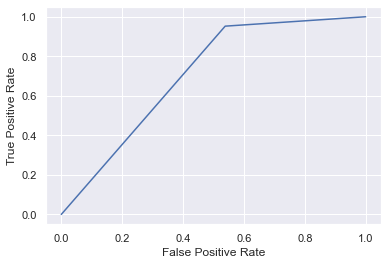
\includegraphics{notebook_files/notebook_60_0.png}
\caption{png}
\end{figure}

\begin{figure}
\centering
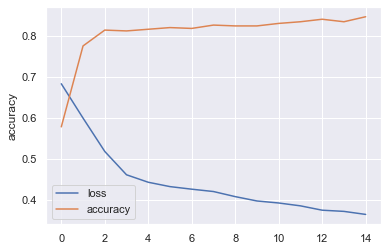
\includegraphics{notebook_files/notebook_60_1.png}
\caption{png}
\end{figure}

RMSE: 0.4508 Accuracy: 0.765 ± 0.199 F1 Score: 0.78

\begin{figure}
\centering
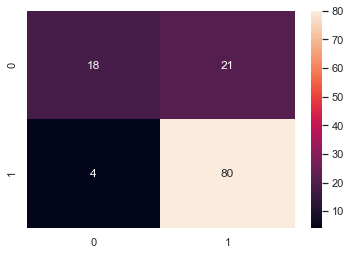
\includegraphics{notebook_files/notebook_60_3.png}
\caption{png}
\end{figure}

Classification Report precision recall f1-score support

\begin{verbatim}
     Y       0.82      0.46      0.59        39
           N       0.79      0.95      0.86        84

    accuracy                           0.80       123
   macro avg       0.81      0.71      0.73       123
weighted avg       0.80      0.80      0.78       123
\end{verbatim}

\hypertarget{evaluation}{%
\subsection{8. Evaluation}\label{evaluation}}

It is easy to see, that we have moved far beyond the perfomance of the
baseline model. Therefore, we could assume our project reached its goal.

From the evaluation metrics it seems, that \emph{deep neural network},
\emph{KNN}, and \emph{SVM} performed nearly equally. Their accuracy
exceeded 80\%. This is quite surprising as \emph{KNN} can be considered
as the most simple from all 4 models and yet it kept pace with them. On
the other side of the spectrum is \emph{decision tree classifier}, which
had the worst evaluation metrics from all 4 models.

And finally, the winner's podium:

\begin{enumerate}
\def\labelenumi{\arabic{enumi}.}
\tightlist
\item
  Deep Neural Network, KNN Classifier, Support Vector Machine
\item
  Decision Tree Classifier
\item
  Dummy classifier
\end{enumerate}

Though keep in mind that with such small dataset the performance of all
models may be influenced by the random state quite a bit.

The performance of all models could be improved in certain models (such
as the DNN classifier) by using weighted samples as the dataset is quite
imbalanced.

The accuracy has quite a large differences between positive and negative
samples. This is most likely caused by the fact that sampling for model
training is not stratified whereas accuracy is computed using stratified
cross validation.

All models seemed to have problems with recognising true negatives. In
all cases the number of false negatives was greater than the number of
true negatives. Though this could be due to imbalanced dataset as well.

\hypertarget{conclusion}{%
\subsection{9. Conclusion}\label{conclusion}}

We have explored and preprocessed the dataset. From the computational
side, training of the models and tuning of their hyperparameters did not
take too long, in average about 35sec per model, with neural network
being an exception, as it was trained with several epochs for each
parameter search. Even though the dataset did not offer many records, we
can conclude that the models performed overall quite well.

\end{document}
